\documentclass[11pt]{amsart}

% Standard letter size paper with 1inch margins
\usepackage[letterpaper, margin=1in]{geometry}
\usepackage{booktabs} % For better looking tables
\usepackage{xcolor}
\usepackage{pifont}

% Useful packages 
\usepackage{amsmath, amssymb, amsthm, amsaddr}
\usepackage{enumerate, subcaption, graphicx, hyperref}
\usepackage{algorithm}
\usepackage{algpseudocode}
\usepackage{cite}
\usepackage{bm}

\newcommand{\I}{\mathrm{i}}
\DeclareMathOperator{\E}{e}

\title{AMATH 582: Homework 5}
\author{Hunter Lybbert} % first and last name

\address{Applied Mathematics Department, University of Washington, Seattle, WA 
\\ \texttt{hlybbert@uw.edu}}

\date{\today} % you can also just type the date instead of "\today"

\begin{document}

\maketitle

\begin{abstract}
    In this report we survey fully connected linear neural networks and the most common hyperparameters to consider for tuning.
    Various methods of optimization are evaluated with a variety of learning rates and momentums.
    Dropout and batch normalization are discussed and implemented as well.
    Methods of hyperparameter tuning, comparing models and results are presented.
    The task we are applying this to is the well known 10 class classification problem with the FashionMNIST dataset.
\end{abstract}

\section{Introduction and Overview}\label{sec:Introduction}
In this report we further our understanding of machine learning concepts focusing on deep learning, the study of neural network based model architecture.

Again, our setup is a common supervised learning problem, given a collection of $N$ data points with labels in classification or target values in a regression setting $$\big\{(\bm{x_0}, y_0), (\bm{x_1}, y_1), ..., (\bm{x_{N-1}}, y_{N-1})\big\}.$$
The data is denoted as a matrix $X$ and a vector of target values or class labels $\bm y$.
We then are looking for a function $f$ which takes in the training data and most accurately predicts the target values or class labels, written in optimization form we are looking for the following
\begin{equation}
f_{MLE} = \underset{f}{\rm argmin } \frac 1 {2 \sigma^2}|| f(X) - \bm y ||_2^2
\label{eq:basic_ml_setup}
\end{equation}
where $\sigma^2$ is the variance of the normally distributed error terms $\epsilon \sim \mathcal N (0, \sigma^2)$ defined by $\epsilon_i = y_i - f(x_i)$
So said another way we are trying to minimize our errors in the classification task.
The specific class of functions $f$ to be considered to solve the problem is a Fully Connected Neural Network (FCN).
We will treat the theoretical background of these methods in the next section \ref{sec:theory}.

Before proceeding, we would like to acknowledge the critical use of the following packages in our analysis.
Namely, Matplotlib was used to create all plots and animations \cite{Hunter:2007}.
Addiitonally, PyTorch \cite{Ansel_PyTorch_2_Faster_2024} was crucial for easily implementing the desired architecture while Ray Tune \cite{liaw2018tune} was used to help with hyper parameter tuning.

\section{Theoretical Background}\label{sec:theory}
For the purpose of this report we will be concise and straight to the point about the methods, architectures, and hyperparameters used in our study.
The motivation for constructing a neural network is quite literally the network structure of the neurons in our very own brains (see Figure \ref{fig:neuron}).

%\begin{figure}[h]
%	\centering
%	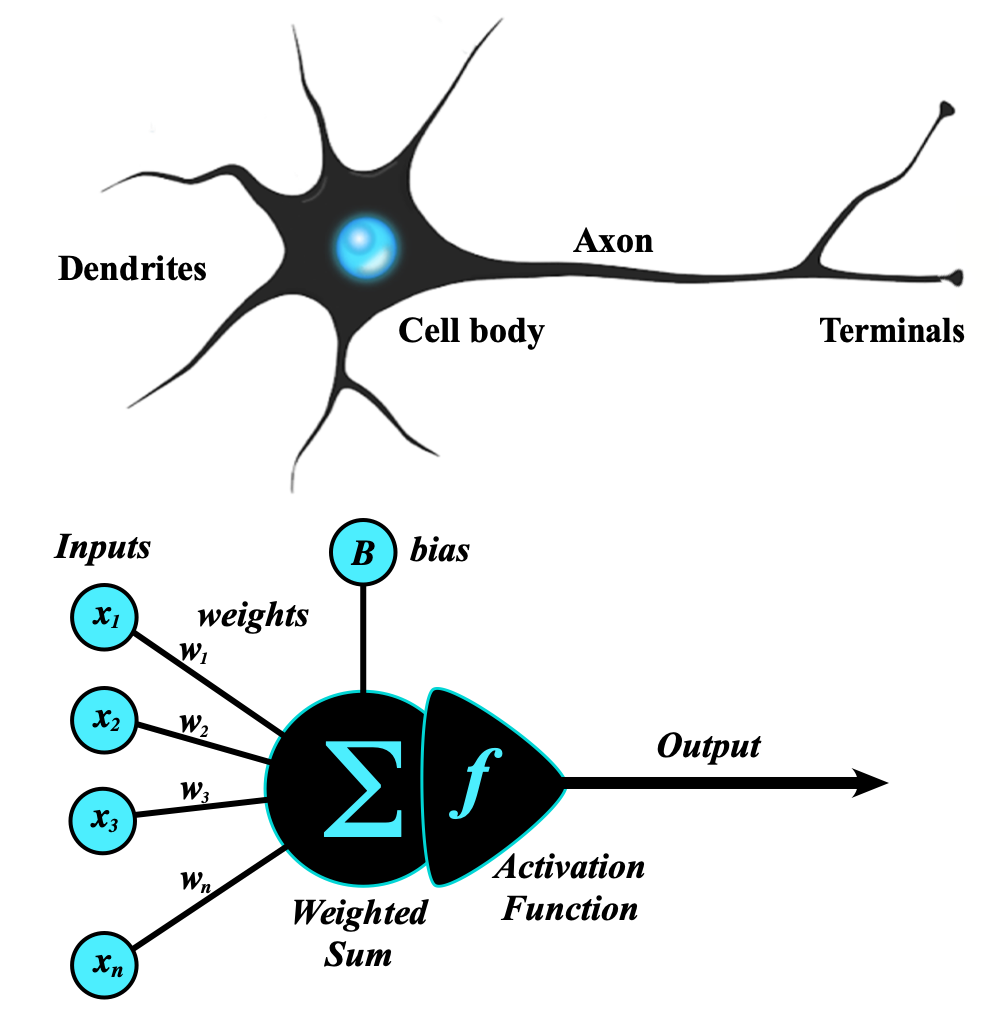
\includegraphics[width=.2\textwidth]{../visualizations/perceptron-with-neuron.png}
% 	\caption{Neural networks are inspired by the biological neurons in our brains \cite{mriquestionsDeepLearning}.}\label{fig:neuron}
%\end{figure}

Key components of a biological neuron which are reflected in the artificial neuron in our models are the Dendrites which receive the signals into the neuron, this is like the weights receiving input from the previous layer.
The Cell body combines these signals like our neuron which calculates a weighted sum of the inputs plus a bias (like in regression).
Depending on the signal a neuron received it may fire and pass along the signal through the axon to the neurons down stream from it, artificially our nonlinear activation functions act as this thresholding decision maker determining when to pass on the signal and at what strength to the next layer.
The power of a neural network is creating a large network that is comprised of very wide layers (many neurons) and or is many layers deep.
However, the basic building block is this artificial neuron we have just described.

Another fundamental piece of information to describe, before we get into the architecture and hyperparameters, is what a forward and backward pass through the network are.
Firstly, a forward pass is simply taking the data we are using to try and make predictions of some sort and passing it into the network.
More mathematically we have the following expression for each neuron
\begin{equation}
y = f\left( \sum_{i=1}^n x_i w_i + b \right)
\label{eq:neuron_calc}
\end{equation}
where $x_i$ are the elements of our input vector $\bm x$  or the results of a previous layers output (past $y$'s).
The $w_i$'s are the weights of the connections between these previous layers outputs or original inputs.
We also add a bias term $b$.
Next, the weighted sum is passed through the nonlinear activation function $f$ to produce either a final prediction if this is the final layer in the network or creating the input for the next hidden (not first or last) layer in the network.
Secondly, a backward pass is when we grade how well the network predicted the target output and we propagate the information about how wrong we were back through the network to improve our prediction a little for the next forward pass.
Once again, we have a more concise mathematical expression for this, which we will get to momentarily.
Recall the expression \eqref{eq:basic_ml_setup} which we are trying to argmin, this metric or measure of error we are trying to minimize is called a loss function.
We can choose different loss functions, let's denote our arbitrary choice of loss function as $L(\hat y, y)$ where $\hat y$ is the predicted label or value from the network and $y$ is the target value or label.
Now we can precisely define backward pass
\begin{equation}
\nabla_{\bm w} L(\hat y, y) = \frac {\partial L}{\partial \hat y} \frac {\partial \hat y}{\partial z} \nabla_{\bm w} z.
\label{eq:back_prop}
\end{equation}
We are referring to variables as represented here in this more graphical representation of forward and backward passes
\begin{align*}
\boxed{\bm w^T \bm x + b = z} \rightarrow \boxed{\sigma(z) = \hat y} \rightarrow \boxed{L(\hat y , y)} \\
\boxed{\nabla_{\bm w} z} \leftarrow \boxed{\frac {\partial \hat y}{\partial z} (z)} \leftarrow \boxed{\frac {\partial L}{\partial \hat y}(\hat y , y)}.
\end{align*}
For completion and yet in favor of being concise, we include the following expression for gradient descent (GD) which is how we update the weights is
\begin{equation}
\bm w_{k + 1} = \bm w_{k} - \alpha \nabla_{\bm w} J(\bm w_{k}; b) \quad
b_{k + 1} = b_{k} - \alpha \frac \partial {\partial b}J(\bm w; b_k)
\label{eq:gd}
\end{equation}
where $\alpha$ is known as the learning rate controlling the size of the step in the direction of the gradient.
There is, of course, more to say about exactly how back propogation works or how autograd works in pytorch but for the sake of this report we will leave it here and begin our discussion of the optimizers and hyperparameters.

\subsection{Architecture}
Deciding the architecture of the model can have large influence on the computational performance and accuracy of your model.
The only considerations after one has decided to use a fully connected network is the number of hidden layers and the size or number of neurons in each hidden layer.
A deeper network can be necessary for some problems but should not be considered the best practice.
One reason to hesitate to use a very deep network is the potential to have vanishing or exploding gradients.
The back propagation across a deep network can begin to get very small causing the optimization to stall and no longer progress.
A wide network can't learn as complex a structure in the data, however, it will train faster and can still do well on small tasks.
A developer needs to make the best decision given their priorities.

\subsection{Optimizer}
There are several variations of gradient descent \eqref{eq:gd} which we are going to describe here.
They each attempt to overcome a few of the challenges with basic gradient descent.

Stochastic Gradient Descent (SGD):
Unlike basic GD which makes updates based on every datapoint in the training set, SGD makes updates more frequently after a batch of data, mini-batch, or even every single datapoint.
The expression for it does not vary enough from the basic one to warrant adding again here.

Adam: 
This adds the ability to vary the learning rate throughout the training process as well as adds a \textit{momentum} term which conveys a sense of certainty that the direction we're moving in is the right one based on where we moved in the previous iteration.
Mathematically this alters equation \eqref{eq:gd} only slightly (for just the weights) we have
\begin{equation}
\begin{split}
\bm v_k &= \eta \bm v_{k-1}  + \alpha \nabla_{\bm w} J(\bm w_{k}; b) \\
\bm w_{k + 1} &= \bm w_{k} - \bm v_k
\end{split}
\end{equation}
where $\eta$ is our momentum parameter which takes on values between 0 and 1 but is commonly close to $0.9$.
Furthermore, our physical intuition for momentum does not lead us astray here.
Imagine, a ball descending down hill, if it has a lot of momentum when it meats a small basin it will likely roll into it and continue out of it if the other side of the basin is not too steep.
If the ball escapes the small basin it will likely continue to descent to an even lower basin and so on until it reaches perhaps the lowest point in the greater region.
Similarly, momentum helps the optimization algorithm avoid local minimums that can trap our methods from arriving at a more globally optimal solution.
We only claim ``more" because it is extremely hard to locate the true global minimum in such a high dimensional nonlinear optimization problem.

RMSProp:
We only mention that this optimizer method exists and was used in our hyperparameter tuning to be discussed later.
As far as the finer details of the method, for our purposes here it suffices to say it is an extended version of AdaGrad which itself introduces an adaptive learning rate.

\subsection{Dropout}
When we train a neural network iteratively on the same training set for many epochs, there is a tendency to overfit.
With regression, we mitigated overfitting with different forms of regularization.
Adding dropout to the model is a neural network form of regularization.
It comes in the form of having some neurons in a particular layer being zeroed out for a particular forward pass.
This forces the model to try and make an accurate prediction without using all of the neurons at once.
The way that this regularizes things a little is that essentially at any one time you are only updating a small portion of the weights essentially creating many sub neural networks within your one network.
These work together to balance one another out and avoid being overfitted to the training data.
Dropout has a parameter in the form of a probability that any one neuron is dropped out for a particular pass.
Different layers can have different probabilities for dropout.

\subsection{Batch Normalization}
This normalizes the output from each layer to be mean 0 and unit variance.
It is calculated as follows:
\begin{equation}
\mu = \frac 1 m \sum_{i = 1}^m z^{(i)}, \quad
\sigma^2 = \frac 1 m \sum_{i = 1}^m \left( z^{(i)} - \mu \right)^2, \quad
z_{norm}^{(i)} = \frac {z^{(i)} - \mu}{\sqrt{\sigma^2 + \epsilon}}
\label{eq:bn}
\end{equation}
Where $\epsilon$ is a parameter used to avoid dividing by 0 and this is calculated over each of the outputs for each batch.
This helps things not explode and get out of hand but it is not a silver bullet.
Really none of these features or parameters are an end all be all, but the combination of them and tweaking them slightly can help improve performance all together.

\subsection{Weight Initialization}
Finally weight initialization is the initial guess to kick off the training process and iterative updates with a form of gradient descent.
An initial guess in optimization can make or break if you will ever find a ``more" globally optimal solution or if you get caught in a local minimum of some kind.
In our class discussion we described that all zeros is a problematic initialization as well as random normal is a poor choice.
A recommended choice from our lectures was Xavier (tanh) which takes the form
\begin{equation}
{\rm Var} ( w^{[l]}): \frac 1 {n^{[l - 1]}}, \quad 
w^{[l]} = N(0, 1) \cdot \sqrt{ \frac 1 {n^{[l - 1]}} }
\label{eq:weight_init}
\end{equation}
We will discuss what our own experiments revealed about weight initialization in our computational results section \ref{sec:results}.

\section{Algorithm Implementation and Development}\label{sec:algorithms}
In order to train a neural network we began by creating a model class using PyTorch's \cite{Ansel_PyTorch_2_Faster_2024} many built in methods and class.
One tricky thing we did was making all kinds of features of our model optional so it required some careful logic to instantiate the model correctly given the architecture and the set of parameters that were specified for the model that iteration.
We wrote a for loop to create any number of hidden layers each of any size of the caller's choice.

Now a crucial part of training the model was managing all of the hyperparameter tuning experiments and recording the statistics for the loss and accuracy across the train, validation, and test sets throughout.
I tried for several days to implement an industry standard tool called Ray Tune \cite{liaw2018tune}.
This proved very challenging to save the model artifact and record the information we needed for each experiment in some logs of sorts.
Therefore, I turned to my own ideas and created an additional python class which managed the experiments for me and recorded results, architecture, and parameter settings to a \textit{json} file which I could inspect later to compare the results of the parameter grid search.
This allowed me to train over 300 models over night and analyze the results the next day and refer back to them in the future as well.
It is all easy to use and very reproducible.

The assignment outline describes iteratively choosing the best setting for each different hyperparameter, but to be more thorough we setup a grid search investigating all combinations of our set of parameters.
The parameters and their eligible values that we used in this grid search is the following:
\begin{align*}
epochs &: [20, 30, 40] \\
hidden \; layer \; dimensions &: [[1024, 256], [1024, 512], [1024, 128]] \\
weight \; initialization &: [\text{xavier\_uniform}, \text{random\_normal}, \text{kaiming\_uniform}] \\
batch \; normalization &: [True, False] \\
activation \; function &: [F.relu] \\
dropout \; rates &: [0.5, 0.3, 0.2, 0.1] \\
optimizers &: [SGD, Adam, RMSprop] \\
learning \; rates &: [0.01, 0.001, 0.0001] \\
momentums &: [0.9, 0.95, 0.99].
\end{align*}
One special note to be made is that we \textit{randomly} selected a pair of values from the dropout rate options for each trial.
In the future, we could perhaps control for this parameter more carefully instead of randomly.
Each experiment was carefully logged and recorded with an experiment number.
Due to the large number of hyper parameters it is an overwhelming amount of information to specify in each plot for each loss or accuracy curve.
Therefore, I have labeled plots with experiment numbers and mean accuracy across test set.
For select models I will detail their exact configuration in the next section \ref{sec:results}, while others can be looked up in the repo directly on \href{https://github.com/hunter-lybbert/uw-central/blob/main/data_analysis/hw_04/experiments/experiments.json}{GitHub}.

\section{Computational Results}\label{sec:results}
We will primarily let the loss, accuracy curves, and hyperparameter configuration tables speak for themselves.
We have included a small sample of the results of our parameter tuning.
Please, see Figures \ref{fig:f0} and \ref{fig:f1} for visualizations of how batch normalization, weight initialization, optimizer choice, and learning rates effected the loss and accuracy curves throughout the training process.
After training our 300 plus models and inspecting which configurations produced a model with above $90\%$ test accuracy, we picked the configuration in \ref{tab:best_model}. We trained a model with this configuration for 5 repeated trials and report the test accuracy mean and standard deviation across trials.
We also repeated this process for the MNIST Digit classification problem from homework 3.
Our best model configuration aligns well with our theoretical background expectations for the optimizer, learning rate, dropout rates, batch normalization, and weight initialization.
A dropout rate around 0.5 was best.
Adam with a low learning rate barely edged out SGD with a larger of a learning rate.
We don't report on RMSprop here (due to space), however, it performed similar to Adam.

We also applied sklearn's $K$-nearest neighbors to this dataset and had a test accuracy of 0.8554 (with number of neighbors set to 5).
Varying the number of neighbors degraded the model slightly.

\begin{table}[h]
    \centering
    \begin{tabular}{|l|c|c|c|c|c|c|c|c|c|c|} % 'l' for left-aligned, 'c' for center-aligned columns
        \hline
        \textbf{Ep.}
        & \textbf{Arch} & \textbf{W. Init}
        & \textbf{B. Norm} & \textbf{Drop}
        & \textbf{Optim} & \textbf{lr}
	& \textbf{$\bm \mu$ (Test Acc)}
        & \textbf{$\bm \sigma$ (Test Acc)} 
        & \textbf{Clasif Prob} \\ 
        \hline
        50 & [1024, 256]  & Kaiming & True & [0.5, 0.5] & Adam & 0.001 & 0.9030 \textcolor{red}{\ding{72}} & 0.0021 & Fashion \\
        \hline
        50 & [1024, 256]  & Kaiming & True & [0.5, 0.5] & Adam & 0.001 & 0.9831 \textcolor{red}{\ding{72}} & 0.0010 & Digits \\
        \hline
    \end{tabular}
    \caption{This is the best configuration that we found. The mean and standard deviation being reported here are with respect to the 5 repeated trials that this configuration was trained for.
    We have included this model configurations performance on the MNIST digits dataset as well.}
    \label{tab:best_model}
\end{table}

%\begin{figure}[h]
%    \centering
%    \begin{subfigure}{0.49\textwidth}
%        \centering
%        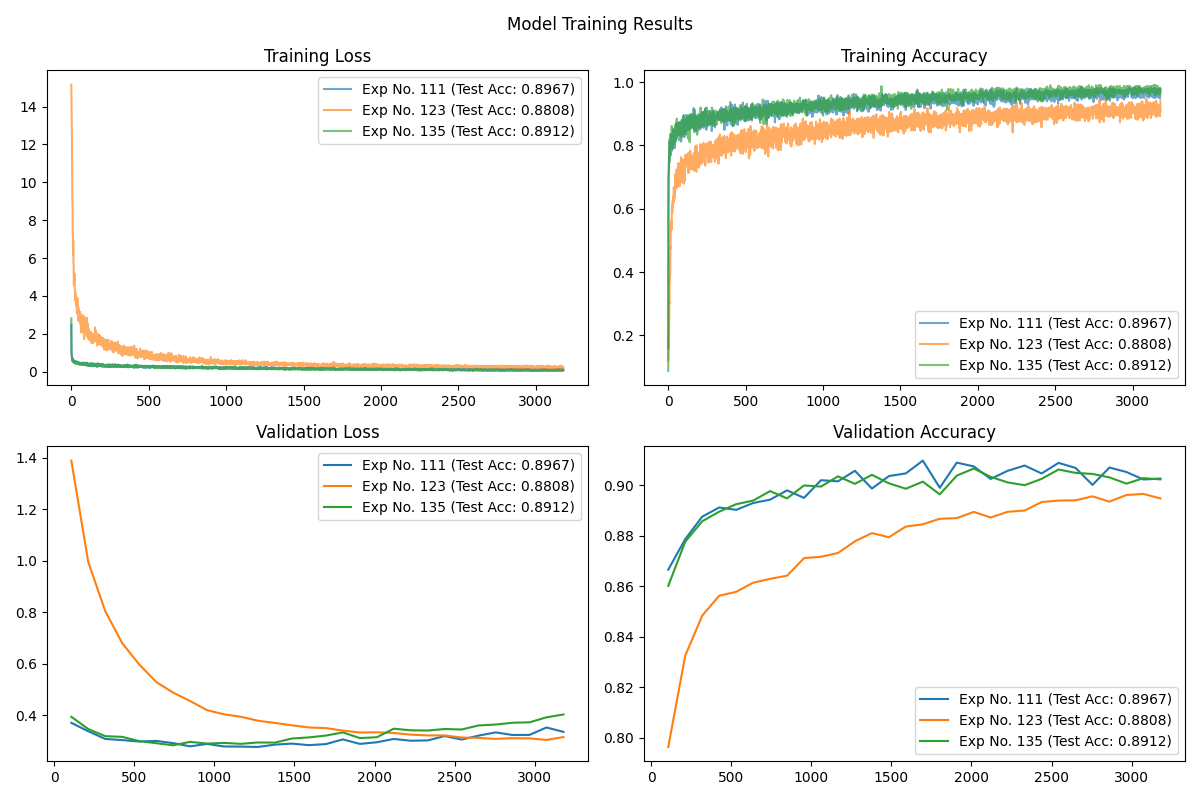
\includegraphics[width=.6\textwidth]{../visualizations/model_training_results_vis_10.png}
%        \label{fig:image1}
%    \end{subfigure}
%    %\hspace{1mm}
%    \begin{subfigure}{0.49\textwidth}
%        \centering
%        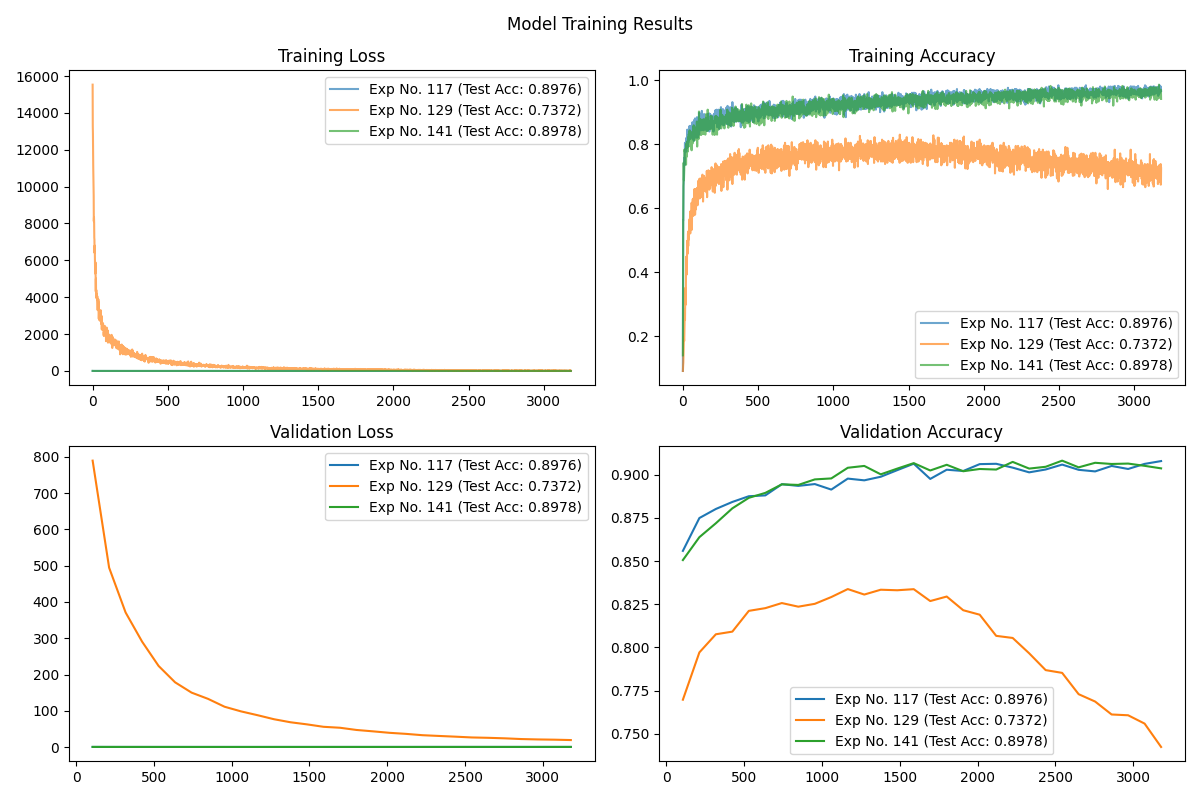
\includegraphics[width=.6\textwidth]{../visualizations/model_training_results_vis_11.png}
%        \label{fig:image2}
%    \end{subfigure}
%    \caption{On the left we have the 3 experiments which are all the same except different weight initializations, compare to Table \ref{tab:tab0}.
%    On the right are these same parameter settings with one change which is that none of them are using batch normalization, compare to Table \ref{tab:tab1}.}
%    \label{fig:f0}
%\end{figure}

\begin{table}[h]
    \centering
    \begin{tabular}{|l|c|c|c|c|c|c|c|c|c|c|} % 'l' for left-aligned, 'c' for center-aligned columns
        \hline
        \textbf{ID} & \textbf{Ep.}
        & \textbf{Arch} & \textbf{W. Init}
        & \textbf{B. Norm} & \textbf{Drop}
        & \textbf{Optim} & \textbf{lr}
	& \textbf{$\bm \mu$ (Test Acc)}
        & \textbf{$\bm \sigma$ (Test Acc)} \\ 
        \hline
        111 & 30 & [1024, 256]  & Xavier 		& True & [0.3, 0.5] & Adam & 0.001 & 0.8967 & 0.0222 \\
        \hline
        123 & 30 & [1024, 256]  & Random N. 	& True & [0.3, 0.2] & Adam & 0.001 & 0.8807 & 0.0202 \\
        \hline
        135 & 30 & [1024, 256]  & Kaiming 		& True & [0.1, 0.1] & Adam & 0.001 & 0.8912 & 0.0175 \\  
        \hline
    \end{tabular}
    \caption{This is a set of 3 experiments where all things are constant except the weight initializations differ.
    See the left hand side of Figure \ref{fig:f0} for a visual of the training and validation loss and accuracy curves.}
    \label{tab:tab0}
\end{table}

\begin{table}[h]
    \centering
    \begin{tabular}{|l|c|c|c|c|c|c|c|c|c|c|} % 'l' for left-aligned, 'c' for center-aligned columns
        \hline
        \textbf{ID} & \textbf{Ep.}
        & \textbf{Arch} & \textbf{W. Init}
        & \textbf{B. Norm} & \textbf{Drop}
        & \textbf{Optim} & \textbf{lr}
	& \textbf{$\bm \mu$ (Test Acc)}
        & \textbf{$\bm \sigma$ (Test Acc)} \\ 
        \hline
        117 & 30 & [1024, 256]  & Xavier 		& False & [0.1, 0.1] & Adam & 0.001 & 0.8976 & 0.0175 \\
        \hline
        129 & 30 & [1024, 256]  & Random N. 	& False & [0.5, 0.3] & Adam & 0.001 & 0.7372 & 0.0335 \\
        \hline
        141 & 30 & [1024, 256]  & Kaiming 		& False & [0.2, 0.5] & Adam & 0.001 & 0.8978 & 0.0251 \\  
        \hline
    \end{tabular}
    \caption{This is a set of 3 experiments where all things are constant except the weight initializations differ.
    Additionally it can be compared to \ref{tab:tab0} since these are the same as those experiments just without Batch Normalization.
    See the right hand side of Figure \ref{fig:f0} for a visual of the training and validation loss and accuracy curves.}
    \label{tab:tab1}
\end{table}

%\begin{figure}[h]
%    \centering
%    \begin{subfigure}{0.49\textwidth}
%        \centering
%        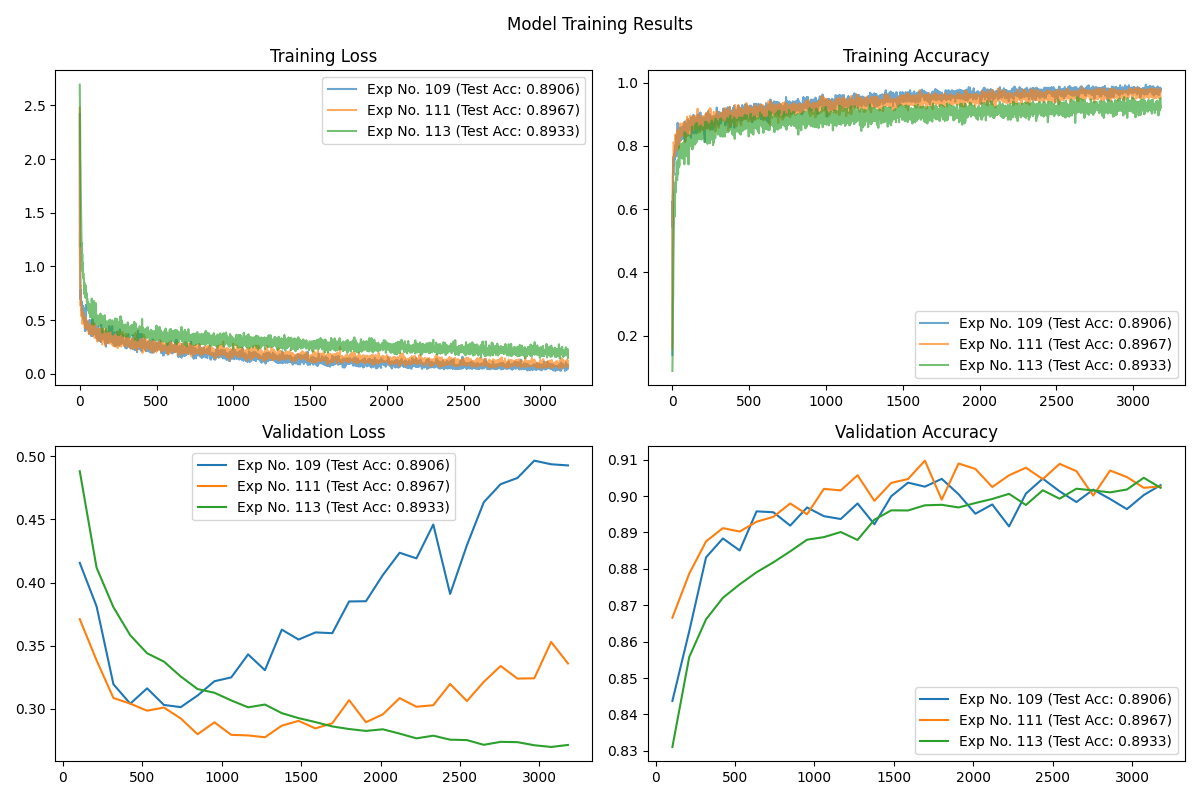
\includegraphics[width=.6\textwidth]{../visualizations/model_training_results_vis_13.png}
%        \label{fig:image1}
%    \end{subfigure}
%    %\hspace{1mm}
%    \begin{subfigure}{0.49\textwidth}
%        \centering
%        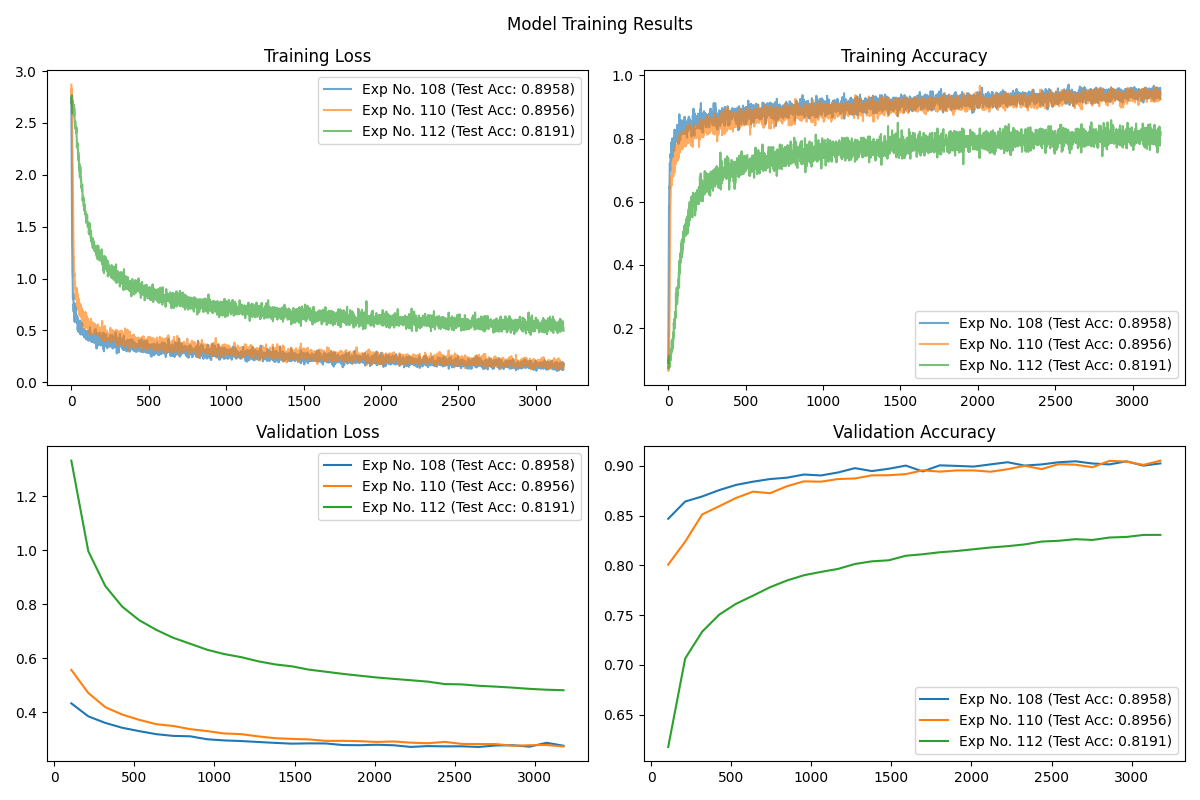
\includegraphics[width=.6\textwidth]{../visualizations/model_training_results_vis_14.png}
%        \label{fig:image2}
%    \end{subfigure}
%    \caption{Here we visualize another set of parameter configurations.
%    On the left we are using the Adam optimizer, while on the right we are using SGD, each with 3 different learning rates.
%    See Table \ref{tab:tab2} for the configurations of the left visual and Table \ref{tab:tab3} for the configurations of the right visual.}
%    \label{fig:f1}
%\end{figure}

\begin{table}[h]
    \centering
    \begin{tabular}{|l|c|c|c|c|c|c|c|c|c|c|} % 'l' for left-aligned, 'c' for center-aligned columns
        \hline
        \textbf{ID} & \textbf{Ep.}
        & \textbf{Arch} & \textbf{W. Init}
        & \textbf{B. Norm} & \textbf{Drop}
        & \textbf{Optim} & \textbf{lr}
	& \textbf{$\bm \mu$ (Test Acc)}
        & \textbf{$\bm \sigma$ (Test Acc)} \\ 
        \hline
        109 & 30 & [1024, 256]  & Xavier & True & [0.1, 0.1] & Adam & 0.01 & 0.8906 & 0.0214 \\
        \hline
        111 & 30 & [1024, 256]  & Xavier & True & [0.3, 0.5] & Adam & 0.001 & 0.8967 & 0.0222 \\
        \hline
        113 & 30 & [1024, 256]  & Xavier & True & [0.5, 0.2] & Adam & 0.0001 & 0.8933 & 0.0189 \\  
        \hline
    \end{tabular}
    \caption{Here all things are constant, including the Adam optimizer, we only vary the learning rate.
    See the left hand side of Figure \ref{fig:f1} for the visualization of this.
    Compare this to Table \ref{tab:tab3} as well to see the same learning rates and config but with SGD.}
    \label{tab:tab2}
\end{table}

\begin{table}[h]
    \centering
    \begin{tabular}{|l|c|c|c|c|c|c|c|c|c|c|} % 'l' for left-aligned, 'c' for center-aligned columns
        \hline
        \textbf{ID} & \textbf{Ep.}
        & \textbf{Arch} & \textbf{W. Init}
        & \textbf{B. Norm} & \textbf{Drop}
        & \textbf{Optim} & \textbf{lr}
	& \textbf{$\bm \mu$ (Test Acc)}
        & \textbf{$\bm \sigma$ (Test Acc)} \\ 
        \hline
        108 & 30 & [1024, 256]  & Xavier & True & [0.3, 0.1] & SGD & 0.01 & 0.8958 & 0.0196 \\
        \hline
        110 & 30 & [1024, 256]  & Xavier & True & [0.2, 0.1] & SGD & 0.001 & 0.8956 & 0.0239 \\
        \hline
        112 & 30 & [1024, 256]  & Xavier & True & [0.5, 0.1] & SGD & 0.0001 & 0.8191 & 0.0293 \\  
        \hline
    \end{tabular}
    \caption{
    Again all things are constant, including the SGD optimizer, we only vary the learning rate.
    See the right hand side of Figure \ref{fig:f1} for the visualization of this.
    Compare this to Table \ref{tab:tab2} as well to see the same learning rates and config but with Adam.
    }
    \label{tab:tab3}
\end{table}


\section{Summary and Conclusions}\label{sec:conclusions} 
In summary, our cully connected network was able to perform pretty well on the FashionMNIST classification task.
Picking the right optimizer with an appropriate learning rate was crucial to improving test accuracy.
Furthermore, weight initialization was perhaps the most volatile parameter, in that choosing random normal initialization dramatically hurt the model's performance, while xavier and kaiming were better if not at least the same as no weight initialization.
We cannot overstate how much time we spent trying to work with ray tune to record experiment results and the challenges that brought on.
In the future, we would like to improve the way we performed our gridsearch and recorded the information.
The method we settled on limited how we could convey the results here in the report, though it recorded thorough information for later reference on \href{https://github.com/hunter-lybbert/uw-central/blob/main/data_analysis/hw_04/experiments/experiments.json}{GitHub}
This was an excellent introductory experience into building, training, and evaluating a neural network.

\section*{Acknowledgements}
The author is thankful to Jaxon Tuggle, Hailey Sparks, Anja Vogt, Jade Glaister, and Nate Ward for offering regular feedback and counsel when interpreting results and clarifying the implications and merits throughout the hyperparameter tuning process.
We would also like to thank Professor Eli Shlizerman for carefully instructing us in class.

\bibliographystyle{abbrv}
\bibliography{references_hw5} % make sure this matches the .bib file for your corresponding document. You also have to maintain your references in the .bib file 

\end{document}
